\documentclass[dvipsnames] {beamer}
\usepackage{cmlgc}
\usepackage{comment}
\usepackage{tikz}
\usefonttheme{serif}     % Font theme: serif
\usepackage[T2A]{fontenc}
\usepackage[utf8]{inputenc}
\usepackage[english]{babel}
\usepackage{amssymb,amsfonts,amsmath,mathtext,cite,enumerate,float} %подключаем нужные пакеты расширений
% \usepackage{cyrillic}
\usepackage{color, colortbl}
\usepackage{multirow}
\usepackage{graphicx}
\usepackage{graphics}
\usepackage{multirow}
\usepackage{url}
\usepackage{hyperref}
\usepackage{animate}
\usepackage{pifont}
\usepackage{wasysym}
\usepackage{marvosym}
\usepackage{appendixnumberbeamer} 
\usepackage{pgfpages}
\usepackage{systeme,mathtools}
\usepackage{mathtools}
\usepackage{listings}
\usepackage{xcolor} % for setting colors
\usepackage{mhchem}


\usepackage{ragged2e} %выравнивание текста по ширине слайда (\justifying)
%\setbeamercolor{background canvas}{bg=violet}

\usetheme{Madrid}
\usecolortheme{crane}

%=================================================

\defbeamertemplate*{footline}{mytheme}{%
  \leavevmode%
  \hbox{%
    \begin{beamercolorbox}[wd=.2\paperwidth,ht=3ex,dp=1ex,center]{author in head/foot}%
      \usebeamerfont{author in head/foot}\insertshortauthor
    \end{beamercolorbox}%
    \begin{beamercolorbox}[wd=.7\paperwidth,ht=3ex,dp=1ex,center]{title in head/foot}%
      \usebeamerfont{title in head/foot}\insertshorttitle
    \end{beamercolorbox}%
    \begin{beamercolorbox}[wd=.1\paperwidth,ht=3ex,dp=1ex,right]{date in head/foot}%
      %\usebeamerfont{date in head/foot}\insertshortdate{}\hspace*{2em}
      %\insertframenumber{} / \inserttotalframenumber\hspace*{2ex} %номер текущего слайда / общее число слайдов
      \insertframenumber{} \hspace*{5ex}  %номер текущего слайда
  \end{beamercolorbox}}%
  \vskip0pt%
}
\usebeamertemplate{mytheme}
\beamertemplatenavigationsymbolsempty

\defbeamertemplate*{frametitle}{boldTitle}{%
  \begin{beamercolorbox}[wd=\paperwidth,ht=3ex,dp=3pt,center]{title in head/foot}%
    %        \ \textit{\textbf{\insertframetitle}} % курсивный заголовок слайда 
    \ \textbf{\insertframetitle}
  \end{beamercolorbox}
}
\usebeamertemplate{boldTitle}
\setbeamercovered{dynamic}

\setbeameroption{hide notes} % Only slides
%\setbeameroption{show only notes} % Only notes
%\setbeameroption{show notes on second screen=right} % Both
%\setbeamertemplate{note page}[plain]


%=================================================
% \titlegraphic{
\includegraphics[width=\textwidth]{logo_conf.png}}

\addtobeamertemplate{title page}{\centering 
\includegraphics[scale=0.5]{meetingLogo.png}}{}
%\addtobeamertemplate{title page}{\centering 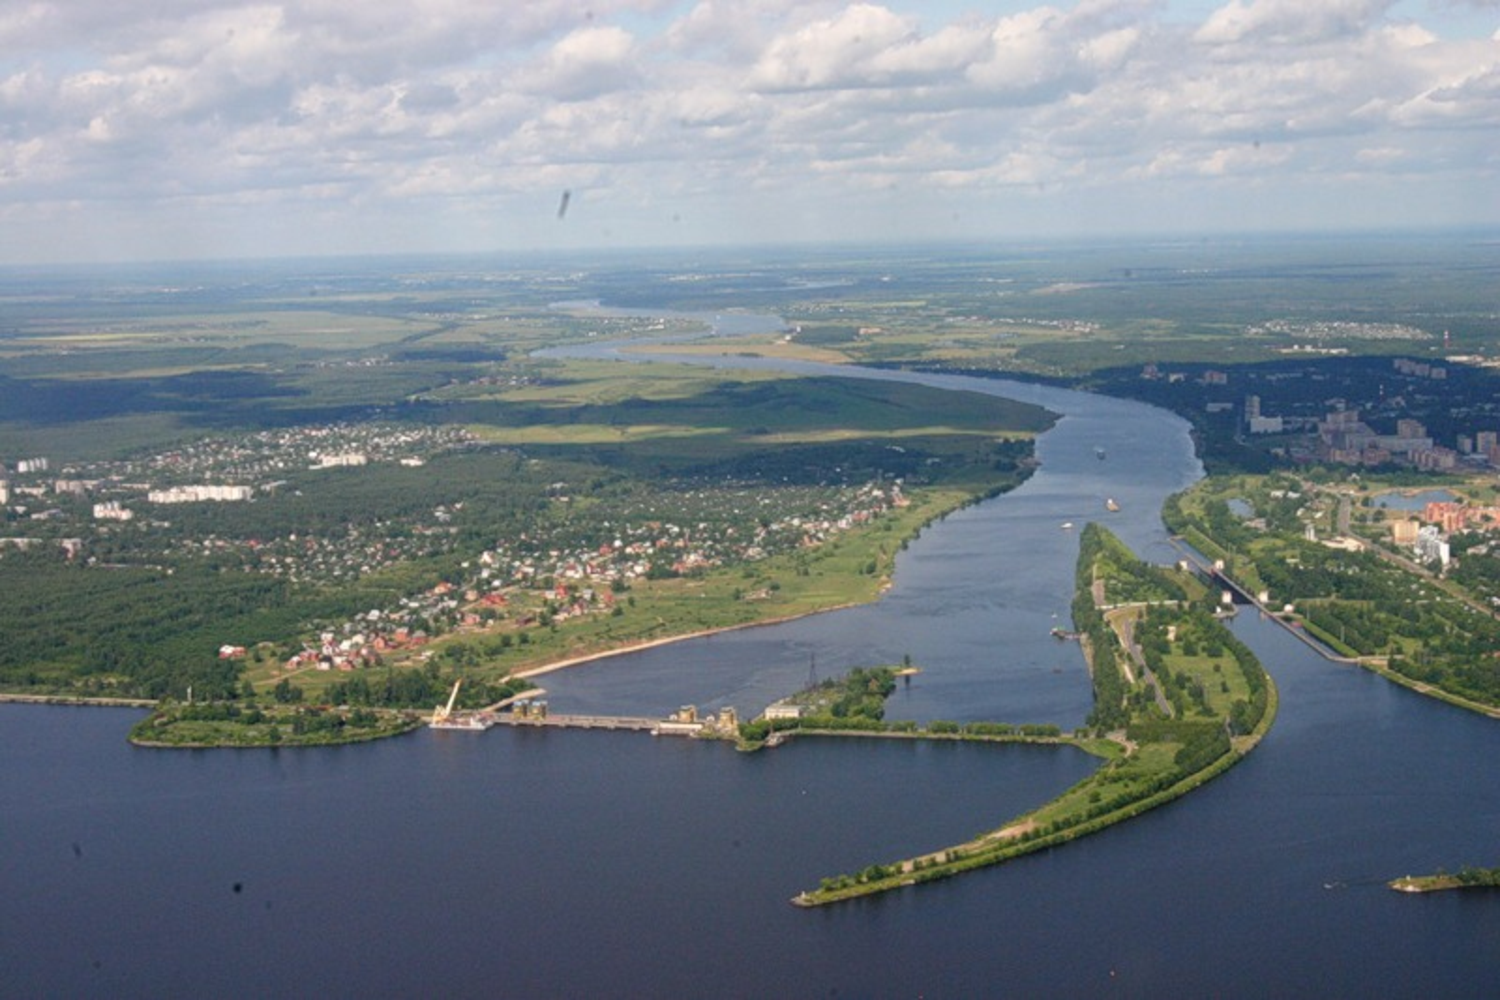
\includegraphics[scale=0.25]{dubna_town.pdf}}{}
%\addtobeamertemplate{title page}{\centering 
\includegraphics[scale=.6]{vblhep_wpcf.png}}{} 
%\addtobeamertemplate{title page}{\centering 
\includegraphics[scale=0.095]{wpcf2018_2.png}}{}

\title[\bf 4th Collaboration Meeting of the BM@N Experiment at the NICA Facility ]{\textbf{\large {Data Offline Quality Analysis in the BM@N experiment}}}

%\author[P.~Batyuk]{\textit{\textbf{{\footnotesize \underline{P.~Batyuk}, L.~Malinina (SINP MSU, JINR), \\ O.~Rogachevskiy (JINR)}}} \\
%  on behalf of the MPD collaboration}
\author[\bf P.~Batyuk]{\textit{\textbf{{\footnotesize \underline{P.~Batyuk}, I.~Gabdrakhmanov}}}} 
%on behalf of the MPD collaboration} 
\institute{\bf Software \& analysis meeting }

\date{{\textbf{October 14, 2019}}}  
% \newpage \footnotesize April 14, 2016}}

\lstset{
  %    frame=tb, % draw a frame at the top and bottom of the code block
  tabsize=4, % tab space width
  showstringspaces=false, % don't mark spaces in strings
  %   numbers=left, % display line numbers on the left
  commentstyle=\color{blue}, % comment color
  keywordstyle=\color{blue}, % keyword color
  stringstyle=\color{red} % string color
}

\graphicspath{{../common_figures/}}

\begin{document}
\maketitle

\begin{frame}
  \frametitle{\bf \centering BM@N RUN6: existing experimental data}
  \begin{block}{\bf \centering Carbon run}
     \begin{figure}[H]
       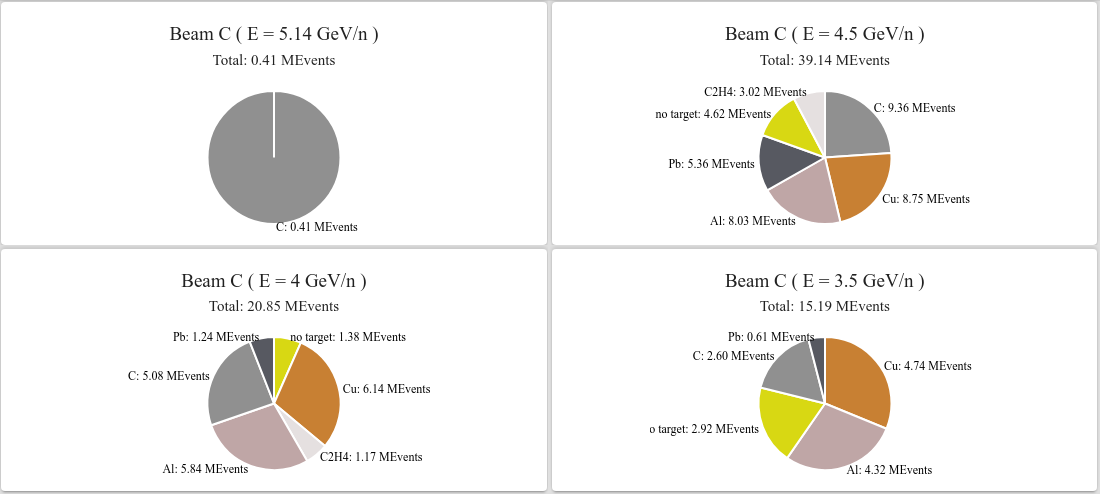
\includegraphics[width=1.\linewidth]{Run6_stat.png}
     \end{figure}
  \end{block}
  \begin{block}{}
    \bf \centering Total amount is about of 75 MEvents 
  \end{block}
\end{frame}

\begin{frame}
  \frametitle{\bf \centering BM@N RUN7: existing experimental data}
  \begin{block}{\bf \centering Argon and Krypton run}
     \begin{figure}[H]
       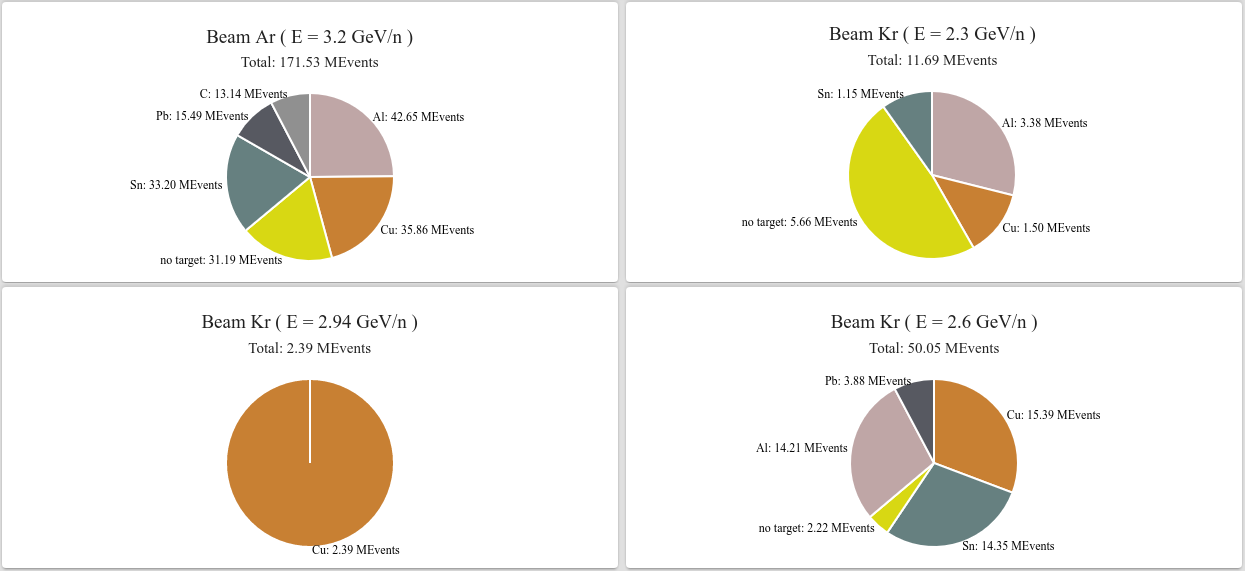
\includegraphics[width=1.\linewidth]{Run7_stat.png}
     \end{figure}
  \end{block}
  \begin{block}{}
    \bf \centering Total amount is about of 237 MEvents \\ (increased by factor of 3 if comparing with RUN6)
  \end{block}
\end{frame}

\begin{frame}
  \frametitle{\bf \centering Types of QA systems to be used}
  \vskip -.4cm
  \begin{columns}
    \column{.49\textwidth}
    \bf
    \begin{block}{\bf \centering {\color{red} Online:}}
      \begin{itemize}
      \item Shows mainly ``raw'' information got directly from a detector system when recording data to be sure of correct working regime of the detector
      \item Allows one to do a comparison between already recorded data
      \item {\color{red} Does not allow one to get a reliable information on high-level data analysis (hits, tracks, physics ...)}
      \end{itemize}
      {\scriptsize \bf See report of I.~Gabdrakhmanov to get more details on}
    \end{block}

    \column{.49\textwidth}
    \begin{block}{\bf \centering {\color{blue} Offline:}}
      \bf
      \begin{itemize}
      \item Has a module structure allowing one to work with different levels of data analysis
      \item Is much more flexible when adding information to be displayed
      \item {\color{red} Makes high-level data analysis more significant since one has some tested versions of alignment, hit producers and track finders...}
      \end{itemize}
    \end{block}
  \end{columns}  
\end{frame}

\begin{frame}
  \bf
  \frametitle {\bf \centering BM@N offline QA-system}
  \begin{block}{\bf \centering Why do we need to use it in BM@N?}
    \begin{itemize}
    \item To see {\color{red} basic distributions} got from existing experimental data {\color{red} for all detectors} (trigger counters, GEM, SILICON, DCH ...)
      whether one relies on a run is being analized or not.
    \item To check hit finders and tracking by basic hit and track distributions (occupancy, reconstructed track parameters, results on matching and PID ...).
      \item Probably, to monitor something else that would require a precise monitoring:)
    \end{itemize}
    \end{block}  
\end{frame}

\begin{frame}
  \bf
  \frametitle {\bf \centering BM@N offline QA-system}
  \begin{block}{\bf \centering What does it do right now?}
    \begin{itemize}
    \item Different histograms are drawn for different detectors (meant those ones I called earlier as ``basic distributions'').
      \begin{itemize}
      \item {\color{blue} Triggers:} {\color{red} Distributions of amplitudes, times, channels.}
      \item {\color{blue} Coordinate detectors (GEM, SILICON, CSC):} {\color{red} Distributions of fired strips per each station, module and layer.}
      \item {\color{blue} Time detectors (TOF, MWPC, DCH):} {\color{red} Distributions of amplitudes, planes, times and strips}
      \item {\color{blue} Calorimeter detectors (ECAL, ZDC):} {\color{red} Distributions of amplitudes and channels}
      \end{itemize}
    \item Basic hit and track distributions got from the tracking developed by our group (S. Merts et. al.). 
    \item All mentioned above can be visualized either for a run we analize ({\color{blue} current}) or couple of them ({\color{blue} current}
    and {\color{red} reference})
    \end{itemize}
  \end{block} 
\end{frame}

\begin{frame}[fragile]
  \bf
  \vskip -0.8cm
  \frametitle {\bf \centering BM@N offline QA-system}
  \begin{columns}[t]
    \column{.43\textwidth}
    \begin{block}{\bf \centering What does it use as an engine?}
      \begin{itemize}
      \item {\color{red} HTTP server in ROOT} (a class called THttpServer)
      \item {\color{blue} Lighthttpd server on host} to provide a {\color{blue} WebUI for users}
      \end{itemize}
    \end{block}
    \begin{block}{}
      \begin{itemize}
      \item {\color{blue} WebUI} displays histograms got from a file produced by
        {\color{red} offline histogram producer} 
      \item Class {\color{red} BmnQaOffline}
      \item Class {\color{blue} BmnQaMonitor}
      \end{itemize}
    \end{block}
    \column{.55\textwidth}

    \begin{block}{\bf \centering \scriptsize offlineQA.C}
          {\tiny 
      \begin{lstlisting}[language=C++,basicstyle=\ttfamily,keywordstyle=\color{red}]
void offlineQA(TString digiFile = "", 
        TString dstBMN = "", 
        TString dstCBM = "", 
        TString out = "", 
        Int_t nEvents) { 

    bmnloadlibs(); // load libraries

    TStopwatch timer;
    timer.Start();
    FairRunAna* fRunAna = new FairRunAna();
    ... 
    BmnQaOffline* qaSystem = new BmnQaOffline(dstBMN);
    fRunAna->AddTask(qaSystem);
    
    fRunAna->Init();
    fRunAna->Run(0, nEvents);
    ... 
}
      \end{lstlisting}
      }
    \end{block}
    \vskip -.3cm
    \begin{block}{\bf \centering \scriptsize startWebServer.C}
        {\tiny 
      \begin{lstlisting}[language=C++,basicstyle=\ttfamily,keywordstyle=\color{red}]
void startWebServer() {
    BmnQaMonitor* mon = new BmnQaMonitor();
    mon->SetHistoDir("/nfs/RUN7_res/QA/output");
} 
      \end{lstlisting}
      }      
    \end{block}
  \end{columns}
\end{frame}

\begin{frame}
  \frametitle{\bf \centering BM@N offline QA-system}
  \bf
   \vskip -.2cm
  \begin{block}{}
    \bf \centering Partially filled with data produced by the BmnRoot software release (19.10.0)
  \end{block}
    \vskip -.7cm
  \begin{columns}[t]
    \column{.3\textwidth}
    \begin{block}{\bf \centering RUN6, BM@N}
      \begin{itemize}
      \item No high-level data put (hits, tracks ...), just ``raw'' information from detectors
      \item  Processed of about of 0.5 kFiles.
      \end{itemize}
    \end{block}
    \column{.3\textwidth}
    \begin{block}{\bf \centering RUN7, BM@N}
       \begin{itemize}
       \item Processed of about of 0.6 kFiles, mainly corresponding to argon part of the run
       \item {\color {red} Shown high-level information is obtained with the current release of software}
      \end{itemize}
    \end{block}
    
    \column{.3\textwidth}
    \begin{block}{\bf \centering RUN7, SRC}
      \begin{itemize}
      \item Processed of about of 1 kFiles.
      \item {\color {red} Shown high-level information is obtained with the current release of software}
      \end{itemize}
    \end{block}
  \end{columns}
\end{frame}

\begin{frame}
  \frametitle {\bf \centering Structure of the BM@N offline QA-system}
  \begin{figure}[H]
    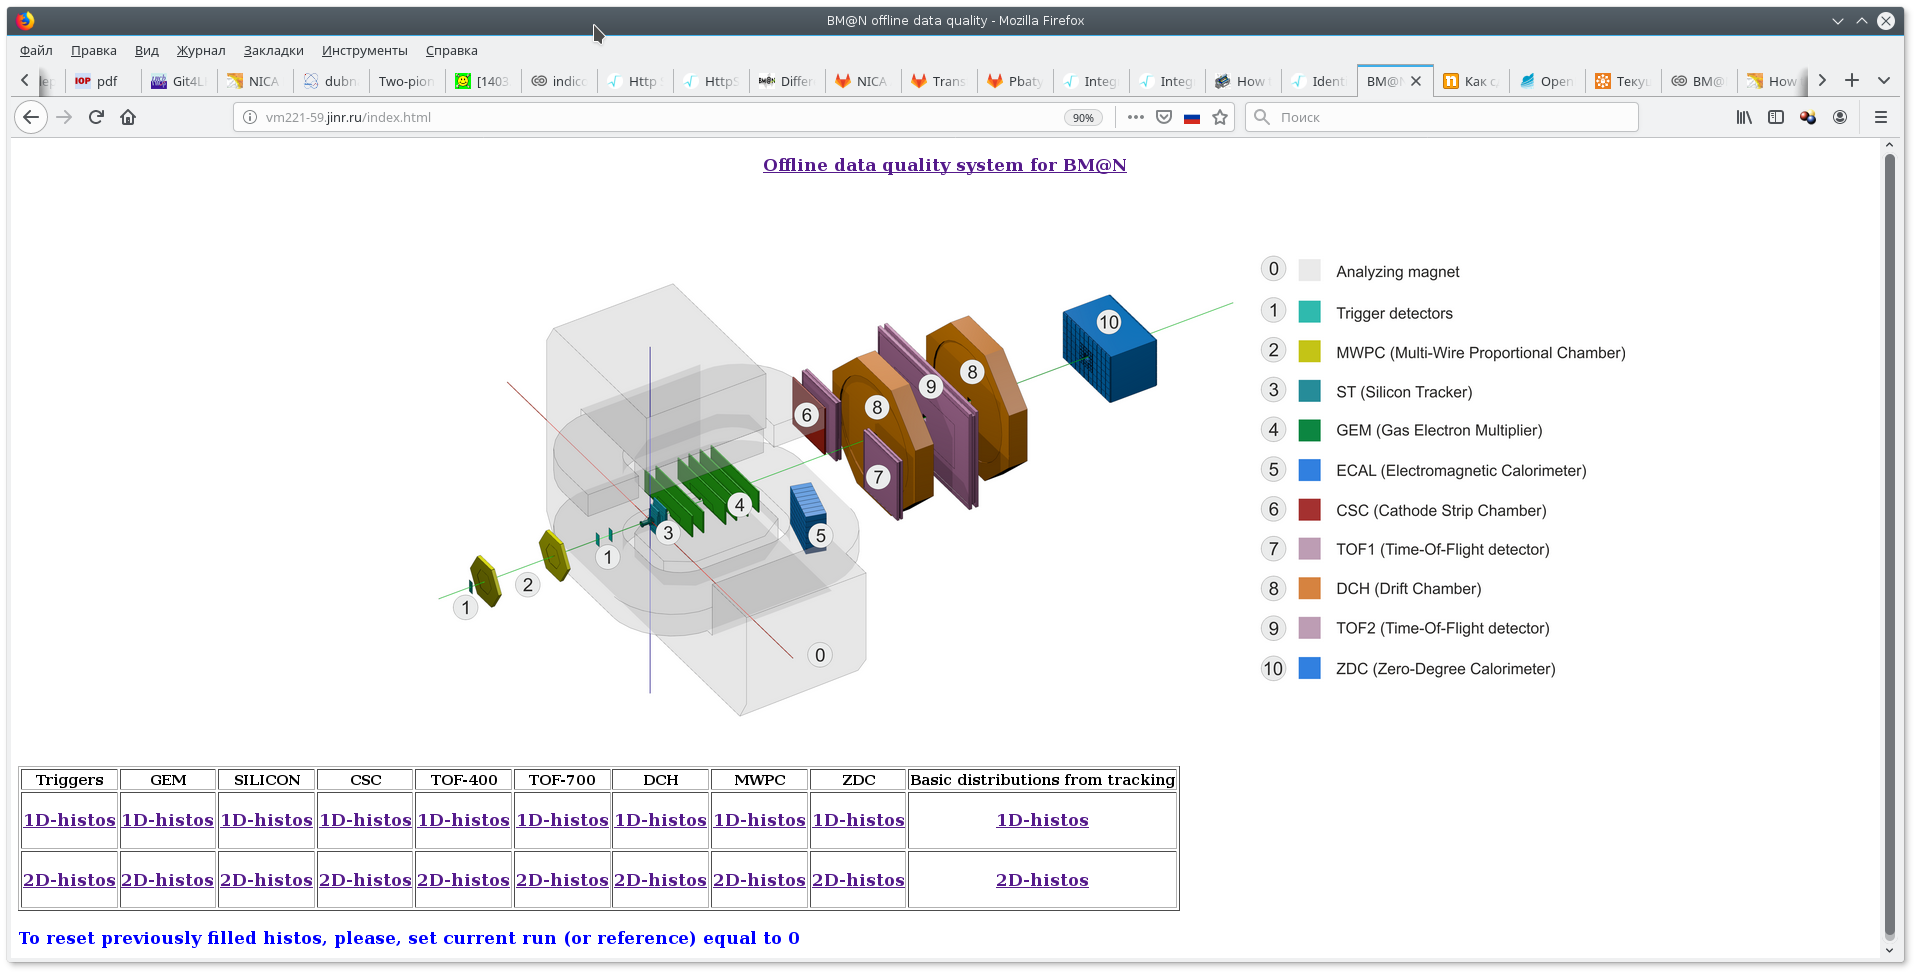
\includegraphics[width=1.\linewidth]{bmaQA_mainPage.png}
  \end{figure}
\end{frame}

\begin{frame}
  \frametitle{\bf \centering BM@N offline QA-system}
  \vskip -.5cm
  %qaOfflineMonExample.png
  \begin{columns}[t]
     \column{.05\textwidth}
    \column{.85\textwidth}
    \begin{block}{\bf \centering {\scriptsize Distributions of basic trigger parameters (amplitude, channels, time ...)}}
    \begin{figure}[H]
       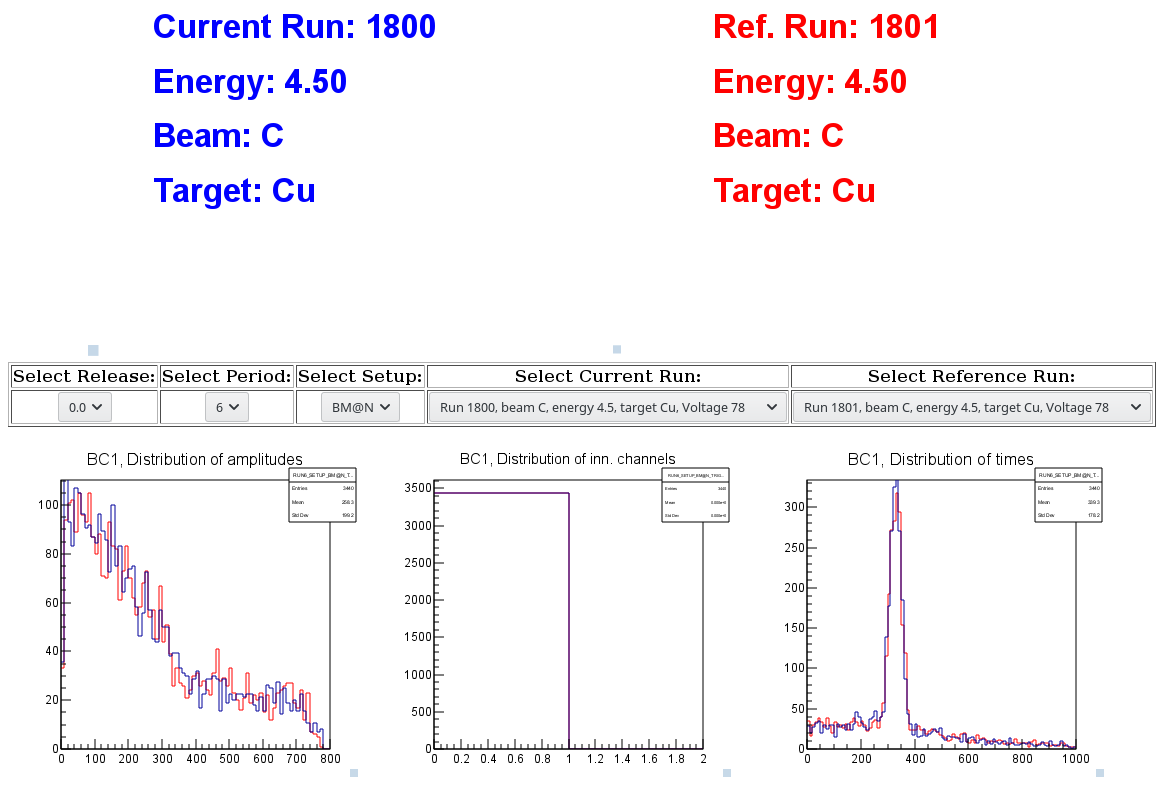
\includegraphics[width=1.\linewidth]{qaOfflineMonExample.png}
     \end{figure}
    \end{block}
    \column{.05\textwidth}    
  \end{columns}
\end{frame}

\begin{frame}
  \frametitle{\bf \centering BM@N offline QA-system}
  \vskip -.5cm
  %qaOfflineMonExample.png
  \begin{columns}[t]
     \column{.05\textwidth}
    \column{.9\textwidth}
    \begin{block}{\bf \centering {\scriptsize Occupancy for SILICON in RUN7 SRC}}
    \begin{figure}[H]
       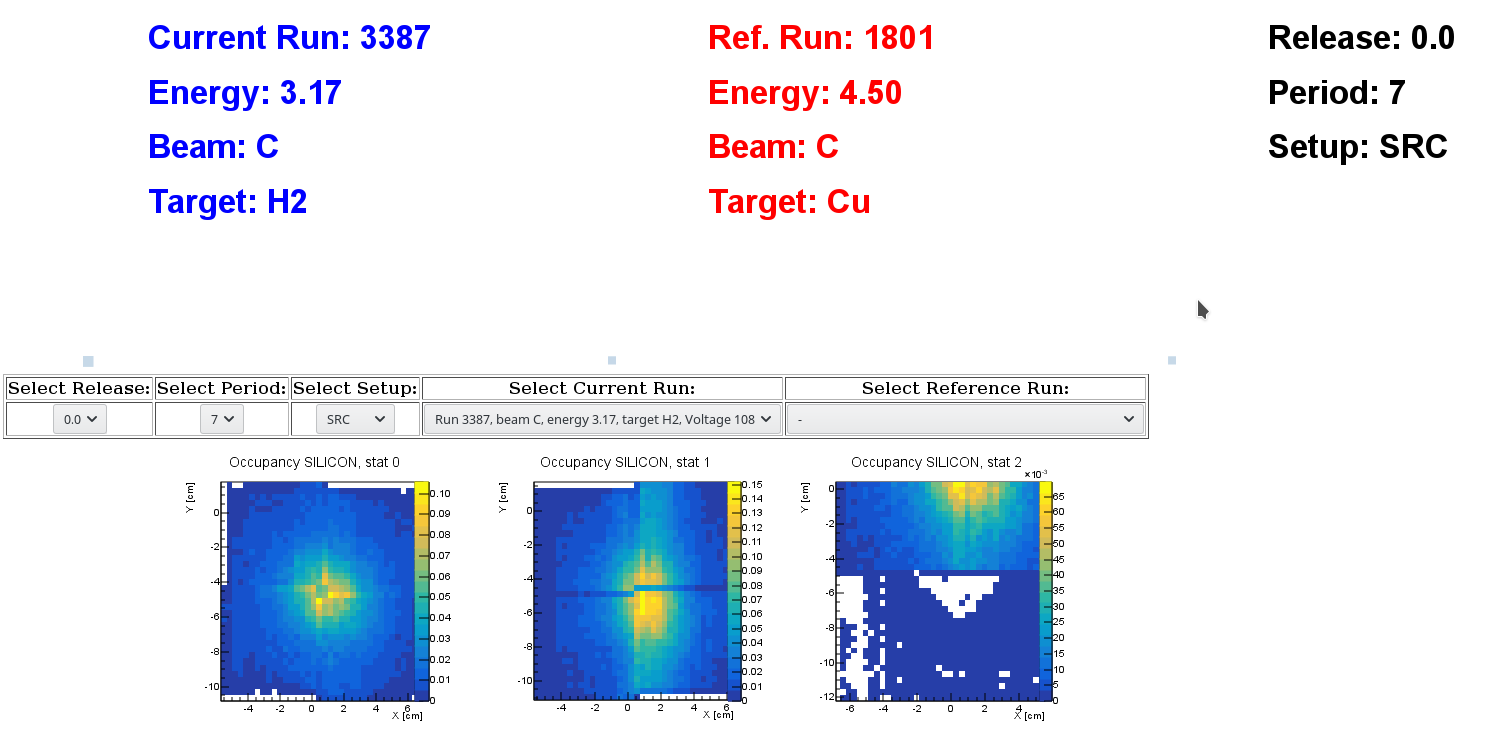
\includegraphics[width=1.\linewidth]{qaOfflineMonExample2.png}
     \end{figure}
    \end{block}
    \column{.05\textwidth}    
  \end{columns}
\end{frame}


\begin{frame}
  \bf
  \frametitle{\bf \centering BM@N offline QA-system, conclusion}
  \begin{block}{}
    It is hosted on {\color{red} vm221-75.jinr.ru} (LIT JINR, cloud infrastructure), probably, to be changed in future to {\color{blue} bmn-qa.jinr.ru}
  \end{block}

  \vskip -.5cm
  \begin{columns}[t]
    \column{.49\textwidth}
    \begin{block}{\bf \centering Already done:}
       \begin{itemize}
       \item {\color{blue} Extended to all possible configurations of BM@N existed}
       \item {\color{blue} Adopted clicking menu to choose release, period, setup ...} 
       \item {\color{blue} Added an useful info canvas with meta-information on runs being analyzed}
       \end{itemize}
    \end{block}
    
    \column{.49\textwidth}
    \begin{block}{\bf \centering To be done:}
      {\scriptsize
      \begin{itemize}
      \item {\color{red} Prepare a stable release of the system}
      \item {\color{red} Add multi-user access}
      \item {\color{red} Extend set of existing histograms and eliminate those ones not representative}
      \item {\color{red} Establish correct binning and histogram ranges for some detectors}
      \item {\color{red} Produce list of shown histograms with their brief explanations}
      \item {\color{red} Improve visibility and usability of the system}
      \end{itemize}
      }
    \end{block}
  \end{columns}
\end{frame}

\end{document}
